\documentclass[conference,a4paper]{IEEEtran}
\usepackage[T1]{fontenc}
\usepackage{amsmath,amssymb,graphicx,booktabs,array,url}
\usepackage[hidelinks]{hyperref}
\graphicspath{{../assets/}}
\hypersetup{pdftitle={VOLLEY: Design and Computational Evaluation of a Commanded Electromagnetic CubeSat Deployment Mechanism},pdfauthor={Adityavardhan Mishra; Pratham Chawla}}
\newcommand{\acr}{Gen5 ACR1}
\begin{document}
\title{VOLLEY: Design and Computational Evaluation of a Commanded Electromagnetic CubeSat Deployment Mechanism}
\author{\IEEEauthorblockN{Adityavardhan Mishra and Pratham Chawla}
\IEEEauthorblockA{Department of Mechanical Engineering\\Symbiosis Institute of Technology\\Symbiosis International (Deemed University), Pune, India}}
\maketitle
\begin{abstract}
Commanded deployment velocity can complement a manoeuvring host when individual CubeSats require different release states. This paper develops and computationally evaluates the Gen5 ACR1 VOLLEY mechanism for twelve 4~kg, 3U envelope surrogates. Two fixed six-cell banks feed a vertically indexed captive pallet that docks to a reusable permanent-magnet carrier. A finite three-phase linear synchronous motor accelerates the payload and carrier, passive cams open the forekeepers before release, and the motor arrests and returns the retained carrier. Eight native/STEP states and 154 accepted motion/refinement checks support nominal geometric compatibility. Represented dry CAD mass is 149.557~kg, with a separate 7~kg power/control allowance. Finite field integration gives approximately 1.328~N/A active force and 1.399~N/A including represented returns; an actual-current finite-element calculation differs by 0.172\% at the checked interior station. An independently audited 5~$\mu$s time-step rerun passes all six principal 3~m/s nominal/adverse and 3/20/100~$\mu$H cases, including source limits and arrest within 210~mm. Actual-carrier elasticity gives 0.286~mm paired magnetic-gap closure under opposed 3.010~kN loads. The results support a computational 1--3~m/s operating study and define an explicit basis for prototype correlation.
\end{abstract}
\begin{IEEEkeywords}
CubeSat deployment, linear synchronous motor, finite magnetic field, payload custody, coupled simulation, computational design.
\end{IEEEkeywords}

\section{Introduction}
A CubeSat deployer must retain a payload before command, establish a repeatable departure path and produce separation compatible with both spacecraft and host. Spring dispensers provide this function with compact mechanisms and operational heritage. Standard interface documents describe the payload envelope and accommodation requirements against which any alternative must be assessed \cite{jssod,cds}. Where a mission requires individual relative release states, deployment velocity becomes an additional control variable.

A manoeuvring host establishes its own state before deployment, while a commanded release establishes the payload state relative to that host. A tangential increment changes orbital energy and period; the benefit depends on the required delivery state and time horizon. Differential drag and host-assisted spring deployment are relevant alternatives, and any comparison must count their resources at a common mission boundary \cite{foster,vallado}. A larger release speed alone does not establish better delivery.

VOLLEY uses a retained moving-magnet carrier driven by an ironless linear synchronous motor (LSM). All added magnetic hardware remains with the host. The payload is represented by a passive 3U envelope and mass surrogate. Reusing the carrier allows successive releases from one motor, but introduces carrier inertia, a post-release arrest requirement and a mechanically significant transfer between storage and launch. Those consequences are included in the reference definition.

The paper evaluates the \acr\ configuration through nominal solid geometry, finite force integration, actual conductor-current modelling, source-coupled dynamics and actual-carrier elasticity. The central question is whether one explicit twelve-payload architecture supports a low-speed commanded operating range when electrical limits and carrier arrest are applied to the same moving mass and geometry. The contribution is the integrated computational reference and its evidence chain. Programmable electromagnetic release and stacked storage are established prior art.

\section{Related Work and Design Basis}
\subsection{Electromagnetic release and storage}
Zhao \emph{et al.} describe a stacked CubeSat deployer with magnetic transfer and multiple release windows \cite{stacked}. Their reported gravity-compensated laboratory releases include approximately 0.67--1.42~m/s for a 1~kg dummy and 0.40--0.85~m/s for a 3~kg dummy over the tested current range. These are physical observations for that mechanism and its test setup. They establish useful test precedents without validating a different motor, interface or payload.

The later high-volume storage study includes stack pushing, receiving guides, magnetic capture and transport \cite{storage}. Its spacecraft-side grooves and iron patches differ from the present passive rectangular-envelope assumption. Its approximately 1200~N receiving contact peaks belong to a zero-gravity simulation, while its faster laboratory pushes use gravity assistance. The distinction motivates separate assessment of endpoint arrival, contact transients and test conditions. Shared-path jams also require containment and explicit recovery conditions.

Feng \emph{et al.} investigate a higher-speed on-orbit electromagnetic launcher and reachable domain \cite{feng}. The acceleration and armature interface differ from the low-speed retained-carrier architecture considered here. Its results provide scaling context rather than a compatible force or velocity rating. The current work concentrates on a complete custody, launch, release and recovery cycle at modest speed.

\subsection{Finite magnetic motors}
The opposed arrays use the field-concentration principle associated with Halbach arrangements \cite{halbach}. A periodic field is useful for initial sizing but does not represent the ends of finite arrays and windings. End effects in Halbach field-magnet linear motors have been studied explicitly \cite{end}. They matter here because the carrier moves from the launch interior toward a finite arrest region, where overlap and available force vary.

The present analysis resolves finite cuboid magnets and actual conductor locations. It independently checks active-conductor force by integrating magnetic source faces, and checks conductor-current assumptions through conduction finite elements. These comparisons target different numerical approximations. They retain shared assumptions about magnet polarization, permeability and the absence of magnetic reaction; physical force validation remains a prototype task.

\subsection{Reference requirements}
The manifest is twelve identical 4~kg 3U surrogates, each 340.5~$\times$~100~$\times$~100~mm. The requirement is a positive custody path from each fixed cell through a shared indexed receiver to a retained carrier. The selected operating study spans 1--3~m/s relative release. The carrier-aft release station is X1500~mm, approximately 1.3~m from the shot origin, followed by 210~mm allocated arrest travel. The host is a generic manoeuvring platform providing charging, attitude control, command/inhibit interfaces and structural accommodation.

A payload envelope is an explicit modelling boundary. Detailed rail contact, permissible loads, magnetic exposure and appendage exclusion require the eventual payload ICD. The study assumes no selected launch provider and makes no provider-acceptance claim. Similarly, supplier data supply reference conditions for source and switching choices; their ratings do not qualify the installed mechanism.

\section{Selected Mechanism and Operating Cycle}
\subsection{Fixed storage and vertical indexing}
Two installed banks contain six dedicated cells each. Guided positive pushers feed a selected payload into the central receiving region. A Z-indexed lift carries the captive pallet, X end frames and independently retracting Y keepers. The central corridor extends 100~mm on either side of Y0; nominal end-frame clearances are 0.5~mm from the payload and relevant carrier corner hardware.

The pallet contains a central crossbar, interleaved payload pads, four 8~mm feet and two outboard lift-grip interfaces. Its feet land on carrier top Z30, while the payload contact plane remains Z46. The same physical pallet is carried by the lift during indexing and retained by the sled during launch, arrest and return. The design therefore does not require a horizontal comb withdrawal drive or a second payload support that is absent from the mass model.

\begin{figure*}[t]
\centering
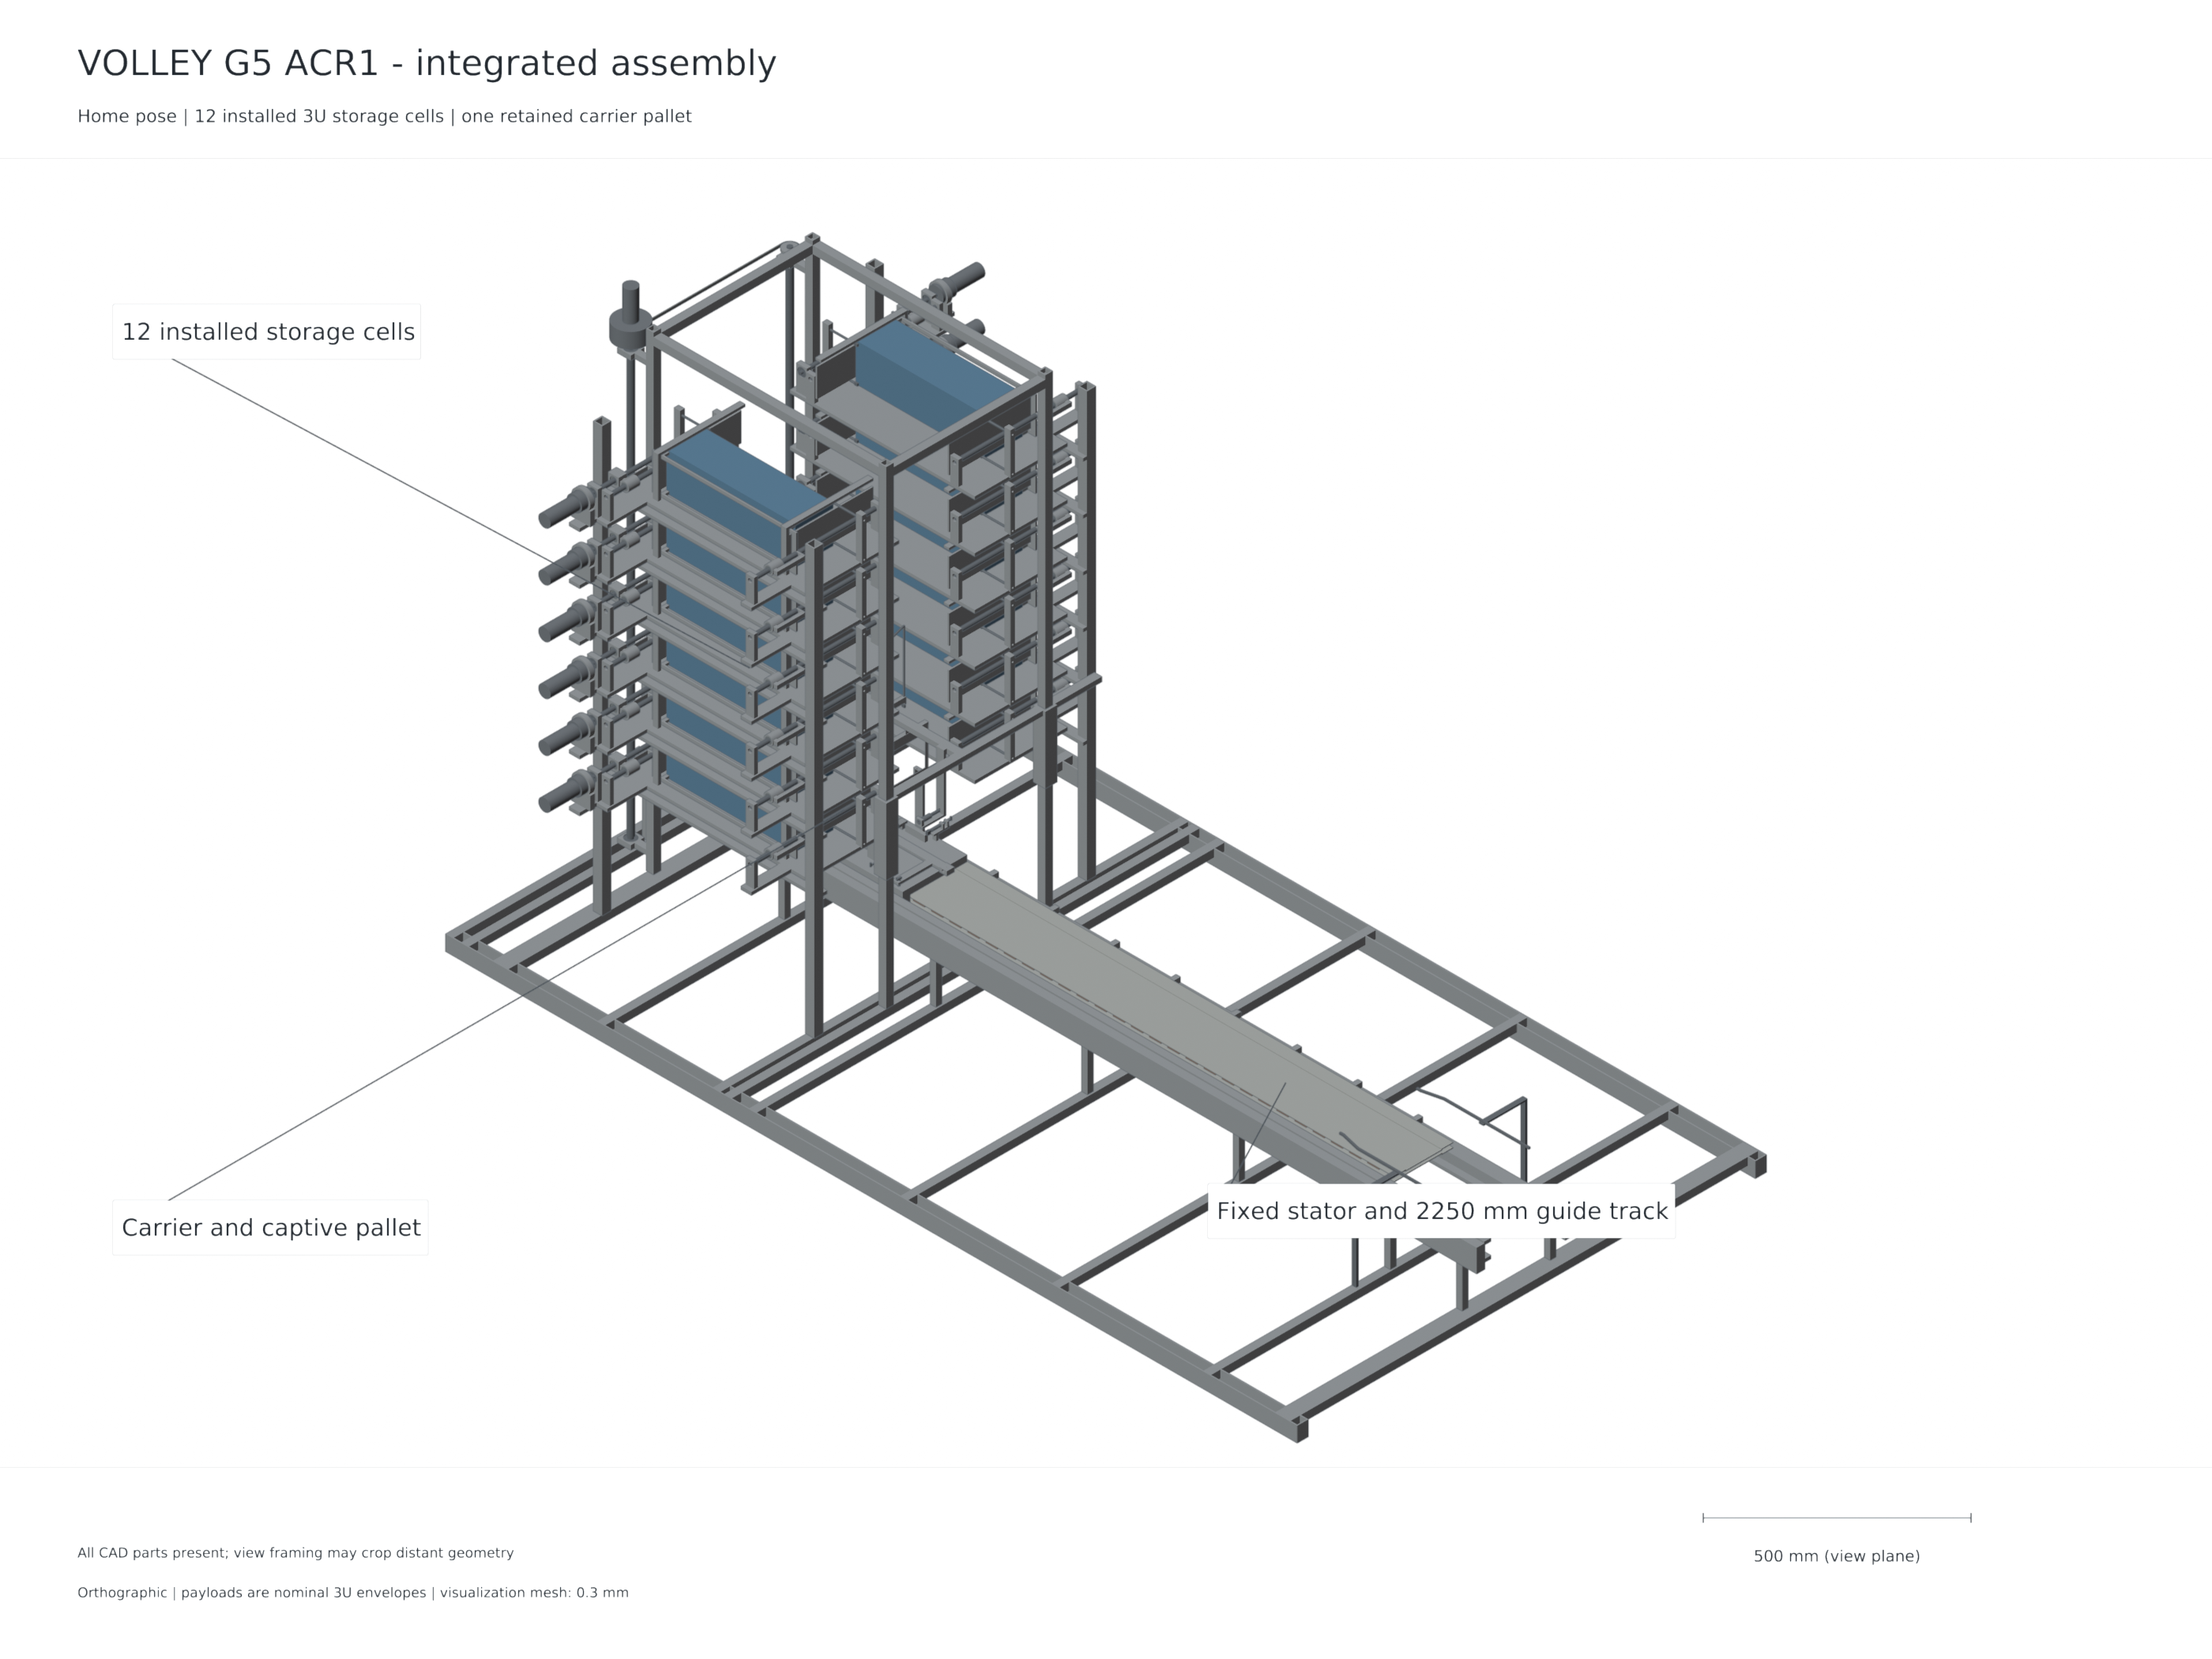
\includegraphics[width=0.76\textwidth]{01_assembly_isometric.png}
\caption{\acr\ native assembly rendered for geometric inspection. Two fixed banks feed a central indexed pallet and shared retained motor carrier. The image represents computational geometry.}
\label{fig:assembly}
\end{figure*}

\subsection{Positive pallet handoff}
Pallet landing occurs while the two outboard lift pins remain engaged. The upper carrier capture caps close and independent lock pins engage. Two 6~mm pallet lock shafts then insert 12~mm through 6.2~mm chassis bores and rotate 12~$\times$~4~mm heads by 90$^\circ$ above the pallet. The locks lie at carrier-local X40 and X468, Y$=-90$~mm. Their heads stow below the pallet underside and rise to the defined capture region when engaged.

Carrier capture precedes overhead-keeper opening and 26~mm withdrawal of the lift grip pins. The lift and end frames then rise clear. Return and pallet retrieval reverse this custody order after carrier home indexing. A separate 6~mm host-index interface must retract before translation. The index locates the carrier at home; the pallet locks retain the pallet during carrier motion.

The lift retains the pallet until the carrier caps and bayonet locks establish capture. The lift grips then withdraw and the lift rises, leaving the carrier in sole custody for the shot. The interlock model encodes this capture-before-release sequence and latches power-loss, jam, sensor-disagreement, timeout and host-burn faults. It accepts 24 nominal commands and passes 166 declared logic tests.

\begin{figure}[t]
\centering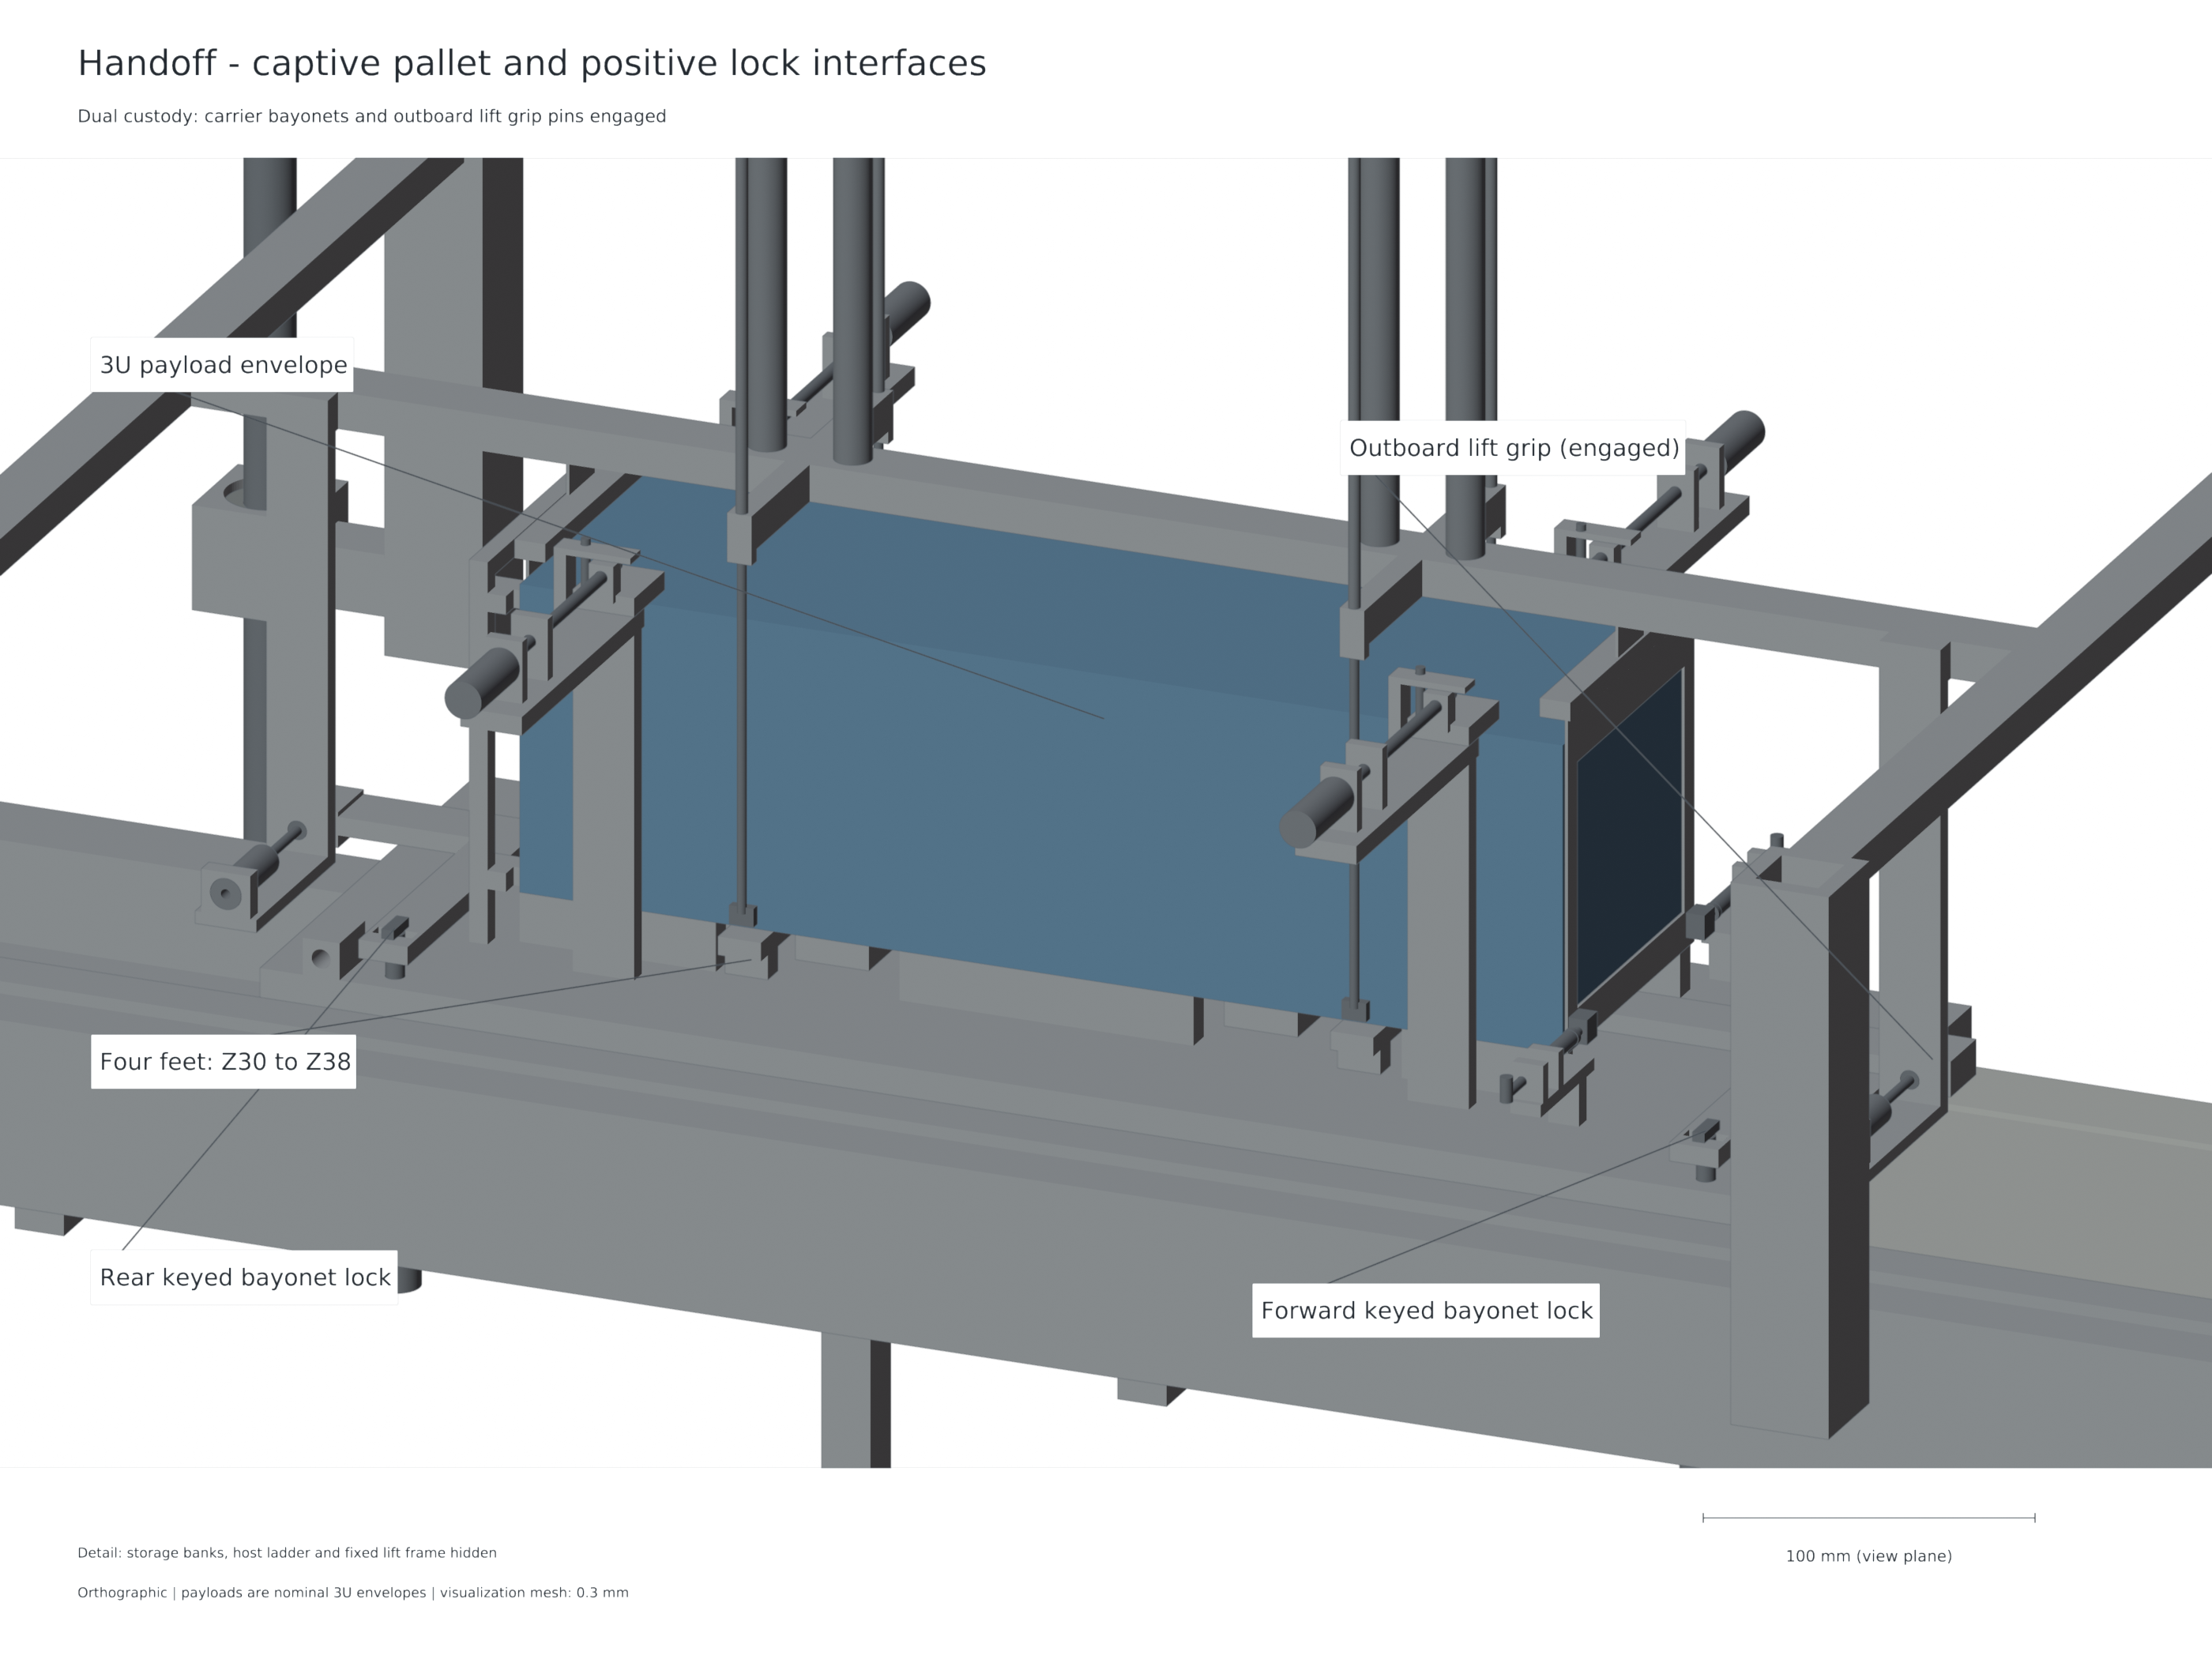
\includegraphics[width=\columnwidth]{02_handoff_pallet_locks.png}
\caption{Pallet handoff. Lift pins remain engaged until carrier capture and pallet locks establish the receiving custody.}
\label{fig:handoff}
\end{figure}

The actual pusher plus payload is 4.201~kg, below the 7.5~kg feed-sizing assumption. Its 250~mm, 40~s quintic command peaks at 11.71875~mm/s. The lift cradle, pallet and payload total 7.573~kg, below the 10~kg lowest lift-sizing case for 784~mm travel in 120~s. Declared coast resistance cases satisfy the catalog and equal-share screw-buckling screens.

\subsection{Finite keeper opening and release}
The forekeepers are spring-closed and open through fixed ramps during the last part of the approach to release. Their 12~mm opening occurs over 50~mm of carrier travel, from carrier-aft X1445 to X1495~mm. The motion finishes 5~mm before the X1500 release station. Rounded followers and a spring reference of 5~N preload with 0.5~N/mm rate define a finite opening process. Open inner edges at $|Y|=54$~mm provide 4~mm side clearance around the nominal 100~mm payload.

Forward pallet ears terminate at Z45.5, 0.5~mm below the payload flight plane. Payload departure is checked to 600~mm relative advance. The loaded carrier accelerates with the payload until the electrical braking command reduces rear-contact normal reaction to zero. The payload then departs; the pallet and magnetic carrier remain on the rail.

The same LSM actively arrests and returns the carrier. At the allocated arrest endpoint the carrier/pallet forward extent is X2224.5~mm, within the 2250~mm rail. No auxiliary eddy-brake force is credited. Arrest is therefore an electrical and mechanical requirement of the selected motor/source combination, rather than an independent idealized catcher assumption.

\begin{figure*}[t]
\centering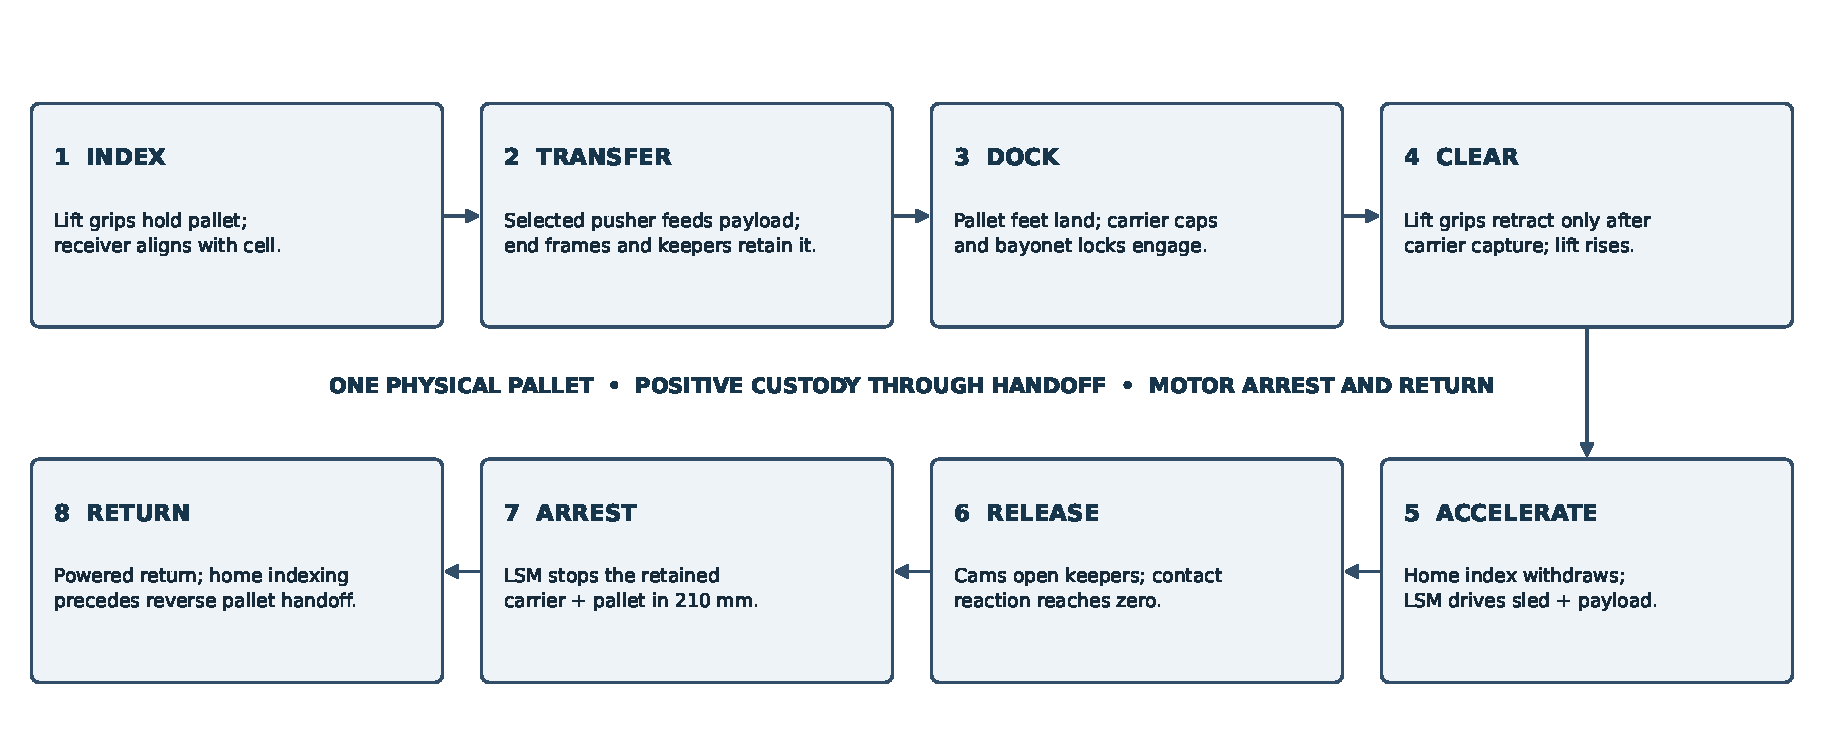
\includegraphics[width=0.97\textwidth]{operating_cycle.pdf}
\caption{Selected operating cycle and custody transitions. One physical pallet passes from the lift to the carrier under positive capture, then returns after LSM arrest.}
\label{fig:cycle}
\end{figure*}

\section{Models and Numerical Methods}
\subsection{Geometry and source identity}
Eight native and STEP states represent home, captured, lower, handoff, withdrawn, clear, release and arrest. The historical filename ``withdrawn'' identifies the grip-pin-withdrawn pose; there is no horizontal pallet-withdrawal motion. Each state records source hashes, named parts, connected-solid checks, interference results and the count of one physical pallet. The native mass ledger uses the released geometry and prescribed material densities.

Accepted motion evidence combines 135 retained baseline poses with 19 direct final checks, for 154. Additional final-refinement reasoning uses strict material subsets, identical closed locks and a conservative full-travel envelope for restored chassis material. These checks establish nominal geometric compatibility of represented parts. Sampled poses do not by themselves establish a continuous collision theorem or manufactured tolerance distribution.

\subsection{Finite-magnet Lorentz integration}
For conductor volume $V_{Cu}$, the longitudinal force is
\begin{equation}
F_x(x,I,\phi)=\int_{V_{Cu}}(\mathbf{J}\times\mathbf{B})_x\,dV.
\label{eq:force}
\end{equation}
The three currents are balanced sinusoids and $I$ is peak phase current. Position-dependent phase coefficients are combined using the specified electrical phase. The force coefficient is consequently in N per peak phase ampere, rather than an unspecified sheet-current convention.

Each opposed array contains 42 discrete blocks at 8~mm pitch and a 48~mm magnetic wavelength, with assumed 1.32~T polarization. The winding has 216 active bars, three connected phase paths and return necks of at least 21~mm$^2$. Active transverse conductors and represented longitudinal returns are evaluated separately. A documented coordinate mapping relates field X travel/Y gap/Z depth to CAD X travel/Z gap/Y depth.

The principal field uses analytical cuboid sources through magpylib \cite{magpylib}. An independent source-face formulation performs magnetic-charge quadrature with exact depth integration for the active conductors. Increasing face order checks convergence of that formulation. A separate conduction solution uses actual connected copper geometry and integrates its finite-element current density against the permanent-magnet field at one interior travel station.

\subsection{Current dynamics and capacitor source}
The effective balanced-current model follows
\begin{equation}
L\dot I_q=V_q-RI_q-K_e(x)v,
\label{eq:current}
\end{equation}
with the production implementation retaining its three-phase power and current definitions. The source is a Thevenin capacitor and ESR. Requested source power must have a feasible physical root and remain within its positive supply limit. During regenerative braking, terminal voltage is limited to $V_{lim}=92.8$~V. With internal capacitor voltage $V_c$ and source resistance $R_s$, the signed power bound is
\begin{equation}
P_{dc}\geq V_{lim}(V_c-V_{lim})/R_s.
\label{eq:regen}
\end{equation}
This enforces the 2.9~V/cell terminal cap in the 32-series source. Phase current, device current, switching-voltage allocation and SVPWM modulation have additional checks. Mean current is supplemented by explicit PWM ripple bounds; the model does not resolve transistor switching.

The reference source is 32S2P Eaton TV1860-3R0107-R family cells, initially charged to 2.7~V/cell or 86.4~V \cite{eaton}. Nominal capacitance is 6.25~F with 0.176~$\Omega$ ESR. The adverse ageing sensitivity uses 3.9375~F and 0.352~$\Omega$. A three-half-bridge inverter contains ten parallel IRFP4668 devices at each switch position, giving 60 devices, and UCC21520 isolated gate-driver references \cite{mosfet,driver}. The 40~kHz PWM model includes hot resistance, a 25\% sharing factor and declared commutation parasitics. These allocations require physical circuit and thermal correlation.

\subsection{Release, arrest and energy balance}
The payload rear contact is unilateral: it transmits compression but cannot pull the payload backward. Electrical braking precedes separation. The release event occurs when computed normal reaction reaches zero. Attached and detached reduced masses are used before and after that event, respectively. This is important because a prescribed instantaneous detach at the brake command would ignore current decay and alter the retained-carrier state.

The finite arrest force map drives the carrier toward rest within the 210~mm allocation. Signed motor work is compared with reduced-mass kinetic-energy change and frictional dissipation. The source ledger includes mechanical, copper, inverter, bank and auxiliary terms, and retains the integration residual. An independently audited time-step rerun refines the production 20~$\mu$s step to 5~$\mu$s for six principal 3~m/s cases. It uses an instrumented copy of the production simulation function, with independent algebra, source-root, limit and conservation checks.

The inductance study includes mutual terms between regularized conductor centrelines. Its refined balanced effective values and radius sensitivities span approximately 4.50--5.82~$\mu$H. The shot model explores 3, 20 and 100~$\mu$H, exposing both ripple and delayed current-decay sensitivity. The larger values are sensitivity cases, not measured winding properties.

\subsection{Actual-carrier elasticity}
The final connected chassis includes 6.2~mm pallet-lock bores, axle bores, integral supports and home lug. The actual BREP is identified byte-for-byte with the selected CAD source. Two 336~$\times$~90~mm patches receive equal 3010.481~N inward loads, integrated over quadratic faces. The opposed pair has zero resultant and moment. Six scalar constraints on three noncollinear web nodes remove rigid-body modes.

Linear elasticity assumes $E=70$~GPa and $\nu=0.33$. Gmsh generates the mesh and CalculiX 2.23 supplies the solution \cite{gmsh,ccx}. Paired face closure is computed at common XY coordinates using quadratic displacement interpolation, avoiding a dependence on arbitrary rigid translation and rotation. A 1.3 load multiplier scales the same linear solution as a sensitivity case.

\subsection{Host and mission boundary}
For payload mass $m_p$, pre-release closed-system mass $M$ and relative release velocity $\mathbf u$, conserved separation gives
\begin{align}
\mathbf v_p&=\mathbf v_0+(1-m_p/M)\mathbf u,\\
\mathbf v_h&=\mathbf v_0-(m_p/M)\mathbf u.
\end{align}
Here $\mathbf u$ is the post-return payload--retained-host relative velocity. With $m_p=4$~kg, retained sled $m_s=13.128$~kg and modeled sled--host release speed $V$, the scalar mapping is
\begin{equation}
u=V\frac{M-m_p-m_s}{M-m_p},\qquad \Delta v_p=V\frac{M-m_p-m_s}{M}.
\end{equation}
Full carrier-mass precision is retained in the inputs. Transient carrier acceleration must be distinguished from final retained-host recoil after arrest. Mission comparisons use a common target state and terminal epoch, propellant model, host-force ceiling and release guards, with architecture-specific retained device mass. They assess the resource effect of commanded release rather than ranking speeds alone. Immediate two-body energy changes are not atmospheric-life predictions.

\section{Results}
\subsection{Geometric compatibility and mass}
All eight released states pass the declared nominal geometry checks. Loaded states contain 387 native parts, and arrest contains 386 after payload departure. One physical pallet is present throughout. The accepted 154 motion/refinement checks support the transfer and launch sequence, including the final lock poses and departure clearances.

The dry represented assembly is 149.557~kg and the twelve payloads add 48~kg, giving 197.557~kg loaded CAD mass. A separate 7~kg power/control allowance gives 156.557~kg dry study mass and 204.557~kg loaded study mass. Sled hardware excluding the pallet is 12.781~kg and the pallet is 0.347~kg, giving the retained moving mass of 13.128~kg used by the shot model.

The 7~kg allowance includes 1.280~kg catalog-typical bare cells and explicit allocations for packaging, protection, switches, drivers, interconnect, cooling plate, charger, controls, harness, supports and reserve. It enters host mass but has no assigned spatial CAD inertia. These are solid-volume and explicit-allocation boundaries. They are not manufacturing estimates with supplier-complete harness, mounting and environmental margins. Dividing dry CAD mass by twelve gives 12.463~kg per carried spacecraft; including the allowance gives 13.046~kg. This substantial retained burden prevents a claim of mass advantage from the current study.

\subsection{Finite force and actual current distribution}
The active force coefficient is approximately 1.328~N/A through the launch interior; represented returns increase it to approximately 1.399~N/A. Increased force quadrature changes active coefficients by approximately 0.100--0.110\% at the checked 0, 0.65 and 1.3~m stations. The refined source-face formulation agrees with the corresponding cuboid active-force values within $10^{-12}$ relative at those stations. The agreement is implementation evidence under shared source assumptions, without physical accuracy at that numerical precision.

At 0.65~m, finite-element current integration over all three actual phase paths gives 1.396651~N/A, compared with 1.399055~N/A from uniform bars and approximate returns. The difference is $-0.1718$\%. It supports the simpler current approximation locally, while retaining limits for centroid quadrature, sharp corners, detailed leads, AC current effects and permanent-field reaction.

\begin{figure}[t]
\centering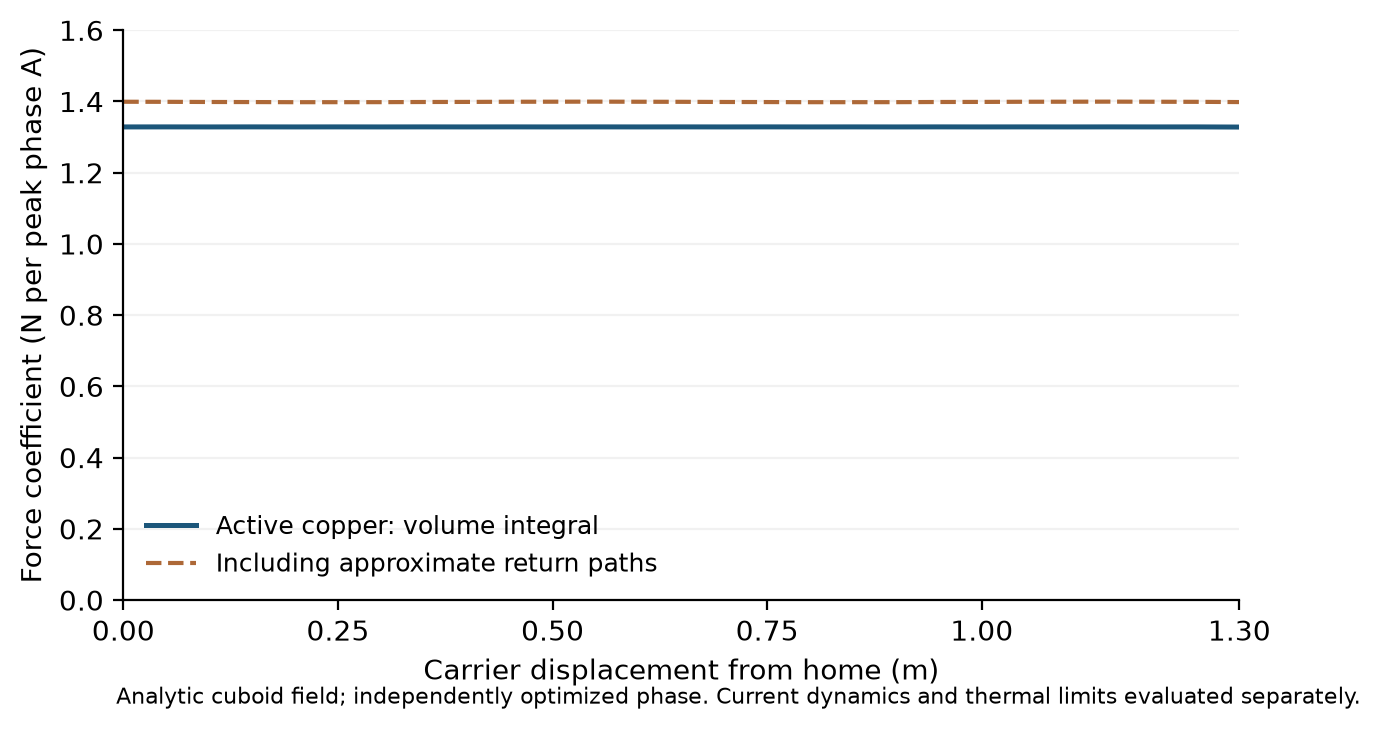
\includegraphics[width=\columnwidth]{finite_force_coefficient.png}
\caption{Finite force-position coefficients from the actual winding and magnet arrangement. Active and represented return contributions are kept distinct.}
\label{fig:force}
\end{figure}

\subsection{Principal source-coupled case}
Table~\ref{tab:shot} reports the independently audited 5~$\mu$s time-step rerun of the six principal 3~m/s cases. All satisfy the declared release speed, source root, positive/regenerative power, mean/ripple current, device allocation, modulation, energy and arrest checks. Stop travel is measured from the launch origin; release near 1.3~m leaves approximately 0.2073~m of post-release motion.

\begin{table}[t]
\caption{Audited Principal 3~m/s Rerun}
\label{tab:shot}
\centering\small
\begin{tabular}{lrrr}
\toprule
Case / $L$ ($\mu$H)&Stop (m)&Peak $I$ (A)&Cell (V)\\
\midrule
Nominal / 3&1.507288637&248.717&2.700000\\
Nominal / 20&1.507288637&248.717&2.725424\\
Nominal / 100&1.507288964&249.246&2.798825\\
Adverse / 3&1.507333466&423.129&2.700000\\
Adverse / 20&1.507333468&423.132&2.899987\\
Adverse / 100&1.507278013&420.040&2.900000\\
\bottomrule
\end{tabular}
\end{table}

The maximum change between 20 and 5~$\mu$s is 0.000670~mm in stop position and 0.0703~A in peak mean current. Maximum electrical energy residual is 0.00247~J. Independently reconstructed kinetic-energy change plus friction agrees with signed motor work within $6.3\times10^{-12}$~J. Actual modulation reaches at most 0.958316 of the ideal SVPWM ceiling. Each capped regenerative step also admits zero requested q voltage, supporting feasibility of the limiting logic.

\begin{figure}[t]
\centering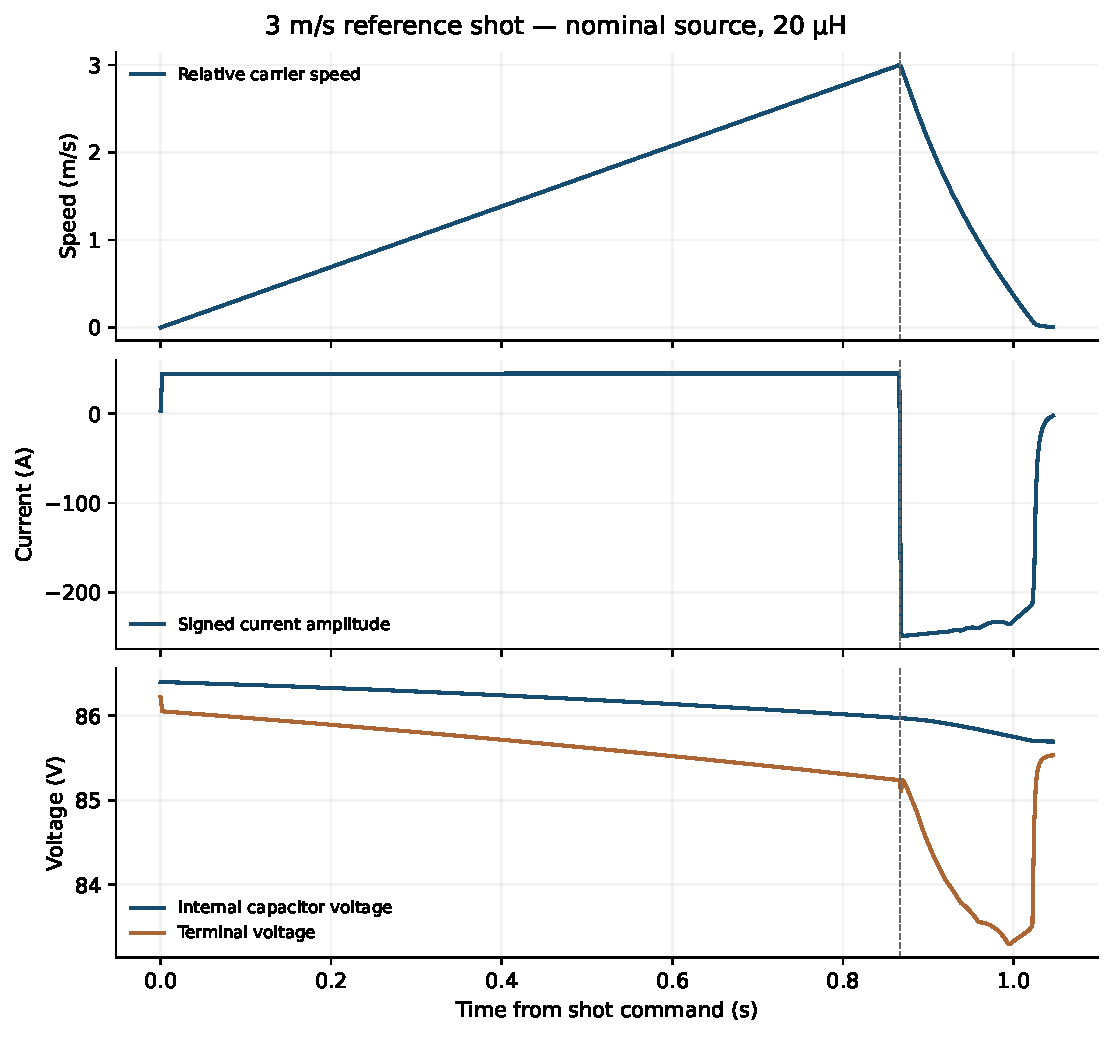
\includegraphics[width=\columnwidth]{coupled_shot_reference.pdf}
\caption{Principal nominal 3~m/s, 20~$\mu$H shot: relative carrier speed, signed current amplitude and internal/terminal source voltages through launch and arrest.}
\label{fig:shot}
\end{figure}

The 1 and 2~m/s commands satisfy the production model checks. The supported computational range is therefore 1--3~m/s, with the complete time-step audit attached to 3~m/s. Higher tested commands do not justify a robust extension above 3~m/s. No 6~m/s rating is assigned.

\subsection{Actual magnetic-gap closure}
The accepted actual-chassis mesh contains 112,519 nodes and 62,198 C3D10 elements, with positive minimum scaled Jacobian 0.075419. Force and moment equilibrium residuals are approximately $1.42\times10^{-12}$ and $1.47\times10^{-12}$ relative to the applied scales. Paired closure is evaluated at 9969 common XY points.

Maximum face-separation reduction is 0.285983~mm at nominal opposed loads and 0.371778~mm under the 1.3 multiplier. The remaining sum of the two nominal 1~mm gaps is 1.714017 and 1.628222~mm, respectively. Positive summed gap is useful for this declared structural comparison; it does not establish both individual assembled gaps. Roller positions, stator-support compliance and alignment enter that separate question.

\begin{figure}[t]
\centering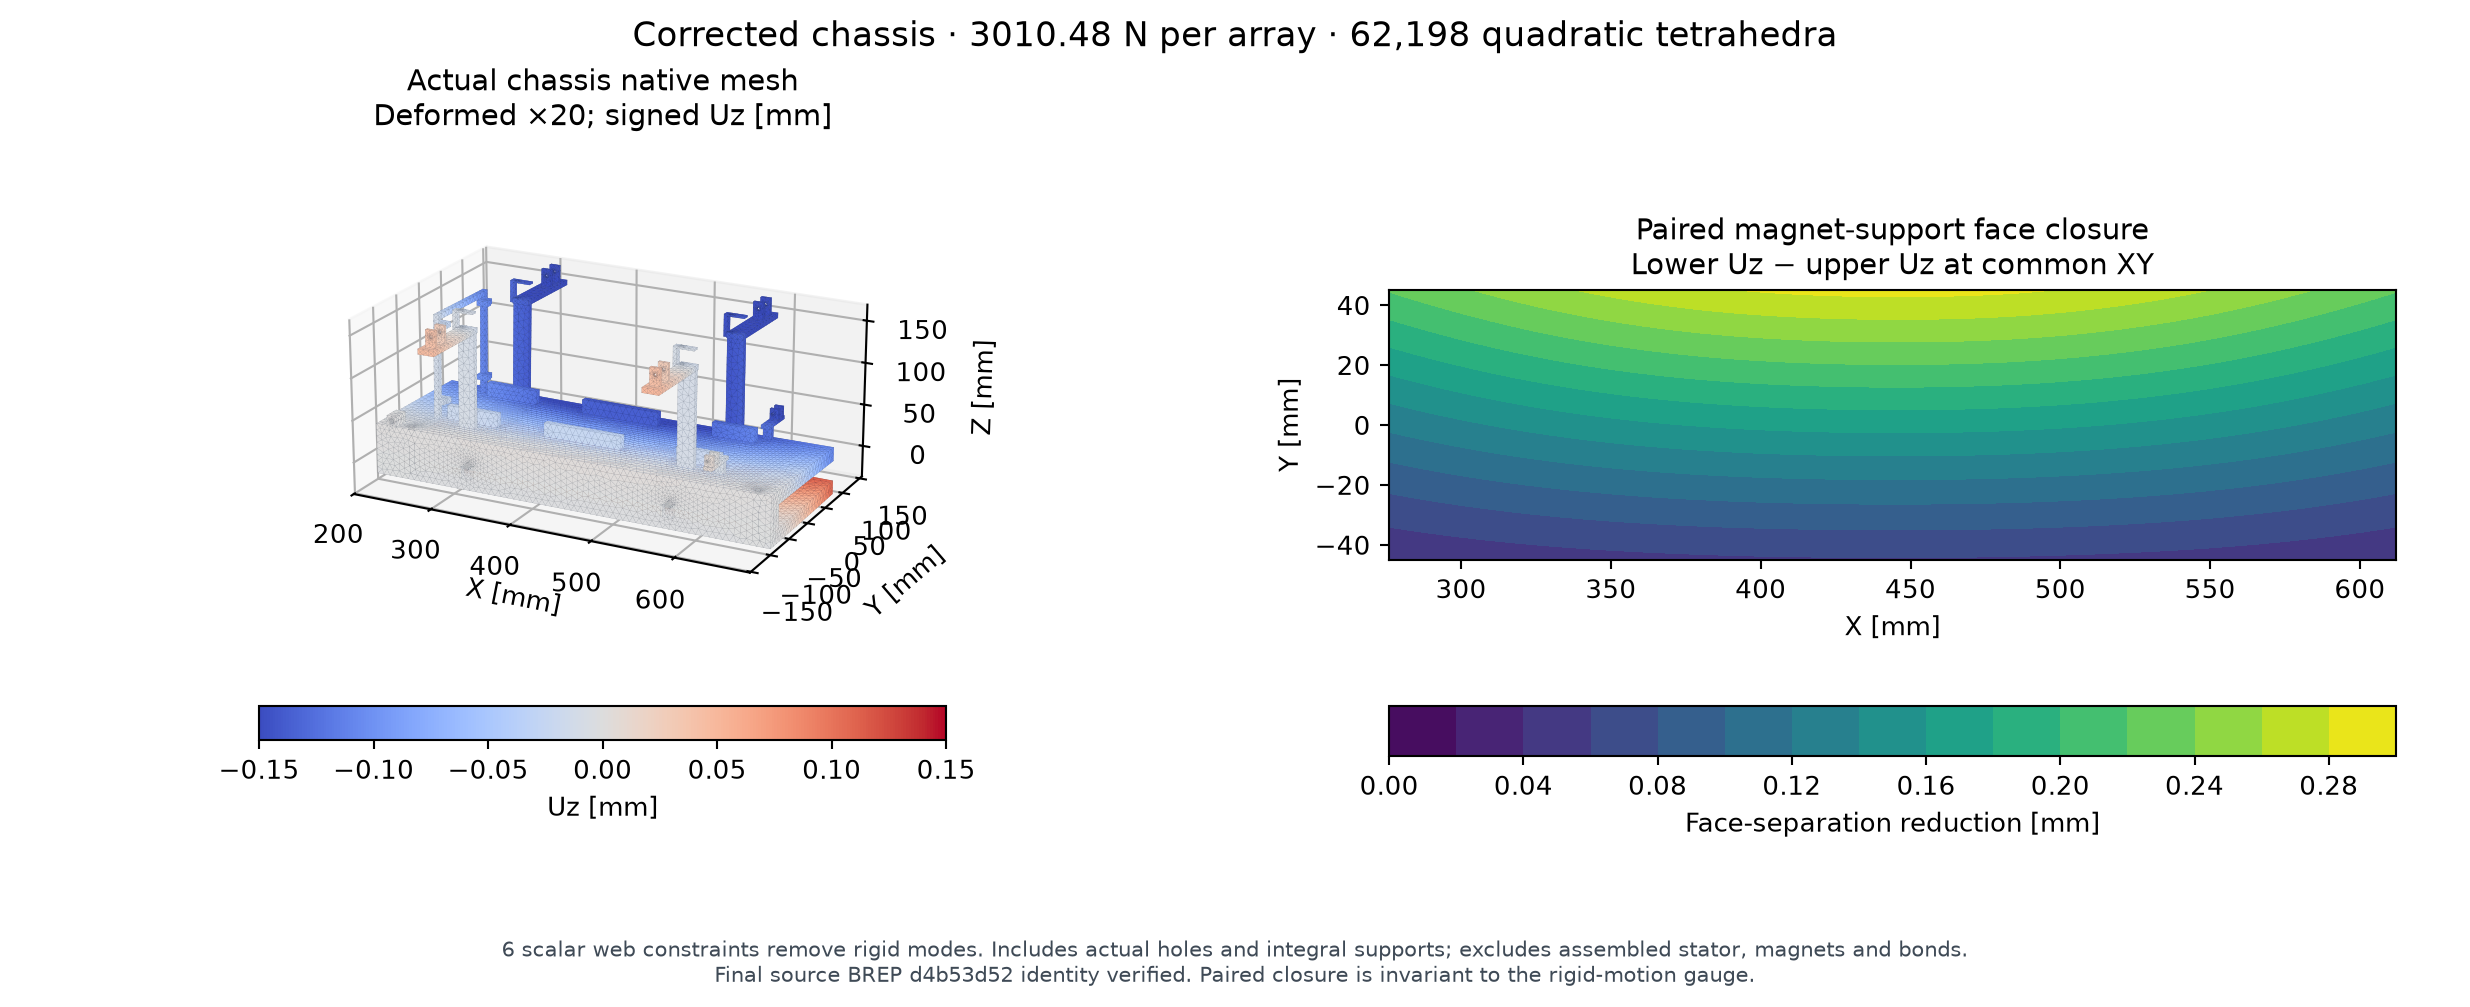
\includegraphics[width=\columnwidth]{ACTUAL_CHASSIS_RESULT.png}
\caption{Actual connected-chassis mesh and paired face closure. Displacement is enlarged for visualization; the reported closure uses common XY sample locations.}
\label{fig:fea}
\end{figure}

\subsection{Clearance and differential expansion}
The individual magnetic-face design budget combines the 1.3-load paired closure with explicit centring, flatness, assembly and thermal allocations. Half the 0.371778~mm closure is assigned to each face about the stated centring bound. Subtracting 0.20~mm guide centring, 0.15~mm flatness, 0.15~mm assembly and 0.05~mm differential thermal movement from each nominal 1~mm gap leaves 0.264111~mm.

For the end-frame rigid stack, the nominal 0.5~mm clearance receives 0.1~mm machining and 0.1~mm docking-repeatability allocations. An assumed differential expansion coefficient of 12~$\mu$m/(m$\cdot$K) over 340.5~mm leaves 0.30000, 0.21828, 0.13656 and 0.05484~mm residual at 0, 20, 40 and 60~K differential temperature, respectively. These positive residuals define the dimensional allocations for subsequent prototype correlation.

\subsection{Conductor heating and repeated operation}
The actual conduction meshes contain 11.061~kg of copper. The calculation assumes heat capacity 385~J/(kg$\cdot$K), density 8960~kg/m$^3$, thermal conductivity 400~W/(m$\cdot$K) and 20$^\circ$C resistivity $1.7\times10^{-8}$~$\Omega$\,m. Bulk heating follows $\Delta T_b=Q_{Cu}/(m_{Cu}c_p)$. Local adiabatic heating uses
\begin{equation}
\Delta T_{local}=\frac{\rho_e}{\rho_m c_p}\int J^2\,dt,
\end{equation}
with the conservative squared-current integral and actual conduction field. Across the eighteen supported 1--3~m/s cases, maximum bulk rise is 0.066668~K per pulse. The volume-99 local estimate is 0.758373~K and the mesh-maximum local observation is 2.495038~K.

A 90~mm repeated-cell diffusion length gives 69.8544~s characteristic diffusion time, compared with 450~s between reference shots. Twelve worst-case pulses with no external-cooling credit give 0.800015~K bulk accumulation. Combining it with one local pulse observation gives a 3.295053~K local recovery estimate under the diffusion assumption. Table~\ref{tab:budgets} collects the principal secondary budgets.

\begin{table}[t]
\caption{Current Secondary Design Budgets}
\label{tab:budgets}
\centering\small
\begin{tabular}{p{0.69\columnwidth}r}
\toprule
Quantity&Result\\
\midrule
Individual magnetic-face allocated margin&0.264111~mm\\
End-frame rigid residual at 60~K differential&0.054840~mm\\
Maximum bulk copper rise per pulse&0.066668~K\\
Mesh-maximum local pulse observation&2.495038~K\\
Twelve-pulse bulk plus one local estimate&3.295053~K\\
Peak payload axial normal reaction&26.863497~N\\
Four-rail pitch/yaw energy bound&1.043585$^\circ$/s\\
Four-rail all-axis energy bound&2.618757$^\circ$/s\\
Nominal free-payload feed-capture energy&0.274658~mJ\\
\bottomrule
\end{tabular}
\end{table}

\subsection{Payload compliance and feed capture}
The peak supported-case payload normal reaction is 26.863497~N. A declared surrogate of four aluminium 8~$\times$~8~$\times$~340.5~mm rails, $E=70$~GPa, and rear-pad compliance gives 51.817~MN/m effective axial stiffness and 6.9634~$\mu$J stored energy. Converting that energy to a selected rotational degree of freedom gives $\omega=\sqrt{2U/I}$. The pitch/yaw inertia of 0.0419801~kg\,m$^2$ gives a 1.043585$^\circ$/s bound; the smallest principal inertia of 0.00666667~kg\,m$^2$ gives the 2.618757$^\circ$/s all-axis bound. One- and two-rail load-sharing sensitivities increase the pitch/yaw bounds to 2.08717 and 1.47585$^\circ$/s, respectively.

Nominal feed capture treats the 4~kg payload as free at the pusher's maximum 11.71875~mm/s speed, giving 0.274658~mJ kinetic energy. Two declared 3~mm steel keeper cantilevers with 118~mm effective length absorb that energy at 0.434927~mm model deflection and 1.26301~N total peak force. This treatment does not assume a gripping connection that would decelerate the payload with the commanded pusher profile.

\subsection{Matched mission}
G5-MISSION-01 uses architecture-independent targets from a common nominal 500~km sun-synchronous chief orbit under fixed-axis J2 gravity. At each release epoch, an inertial along-track 1, 2 or 3~m/s increment is added to the chief state and propagated to a common terminal epoch. One family uses uniform 2~m/s increments and the other alternates 1 and 3~m/s. VOLLEY release states use the current source-coupled calibration and conserved retained-carrier mapping.

The host starts at 500~kg wet mass: 480~kg dry bus and 20~kg propellant, with 220~s specific impulse. Including the 48~kg manifest gives 704.557~kg initial mass for VOLLEY and 620~kg for a declared 72~kg spring device-class reference. Twelve releases occur from 450 to 5400~s in 450~s slots; the final epoch is 91800~s, 24~h after the last release. Both options have 5~s pre-release and 20~s post-release zero-force guards. VOLLEY's 400~s loading coast contains a 355~s declared cycle and 45~s reserve. Spring candidates can also use wider manoeuvre windows, with no inherited VOLLEY loading constraint.

The conventional benchmarks are a fixed 2~m/s separation class and ideal per-payload pretrim, which sets separation energy before the campaign to compensate predictable recoil. Pretrim supplies no in-flight retasking. Fourteen target-closed candidate policies are screened at 1 and 5~N host ceilings. Table~\ref{tab:mission} reports the least-propellant tested candidates within each ceiling.

\begin{table}[t]
\caption{Current Matched-State Mission Candidates}
\label{tab:mission}
\centering\small
\begin{tabular}{llrr}
\toprule
Family / ceiling&Policy&Fuel (kg)&Peak (N)\\
\midrule
U2 / 1 or 5~N&VOLLEY&0.0524&0.677827\\
U2 / 1 or 5~N&Fixed-2&0.0470&0.656269\\
U2 / 1 or 5~N&Pretrim&0.0524&0.677826\\
A13 / 1~N&Pretrim, wide&0.0750&0.184432\\
A13 / 5~N&VOLLEY&0.2899&4.204212\\
A13 / 5~N&Pretrim, shared&0.0536&1.016738\\
\bottomrule
\end{tabular}
\\[3pt]\parbox{\columnwidth}{\footnotesize U2: uniform 2~m/s targets. A13: alternating 1/3~m/s targets. ``Shared'' uses the common narrow windows; spring may also select wider windows. Device masses: VOLLEY 156.557~kg; spring 72~kg class assumption.}
\end{table}

No tested VOLLEY or fixed-2 candidate meets the alternating-family 1~N ceiling. VOLLEY closes at 5~N; the smallest tested fixed-2 peak is 7.537264~N. This candidate result is not global infeasibility: ideal pretrim closes both force cases. In the uniform family, VOLLEY and pretrim have closely similar fuel demand. In the alternating 5~N family, VOLLEY uses 0.2899~kg versus 0.0536~kg for pretrim. Combined with an 84.557~kg device penalty, the current result establishes no mass or fuel advantage over the ideal pretrim benchmark.

Nine native Orekit replay jobs comprise six nominal bounded cases, one above-ceiling diagnostic and two refinements \cite{orekit}. All declared numerical checks pass. The worst native target differences are 11.247~$\mu$m and $1.235\times10^{-8}$~m/s; independent mass-flow and momentum residuals remain below $1.26\times10^{-12}$~kg and $1.05\times10^{-9}$~kg\,m/s. Reducing maximum step from 60 to 30~s changes the checked VOLLEY terminal positions by at most 12.178~$\mu$m.

\begin{figure*}[t]
\centering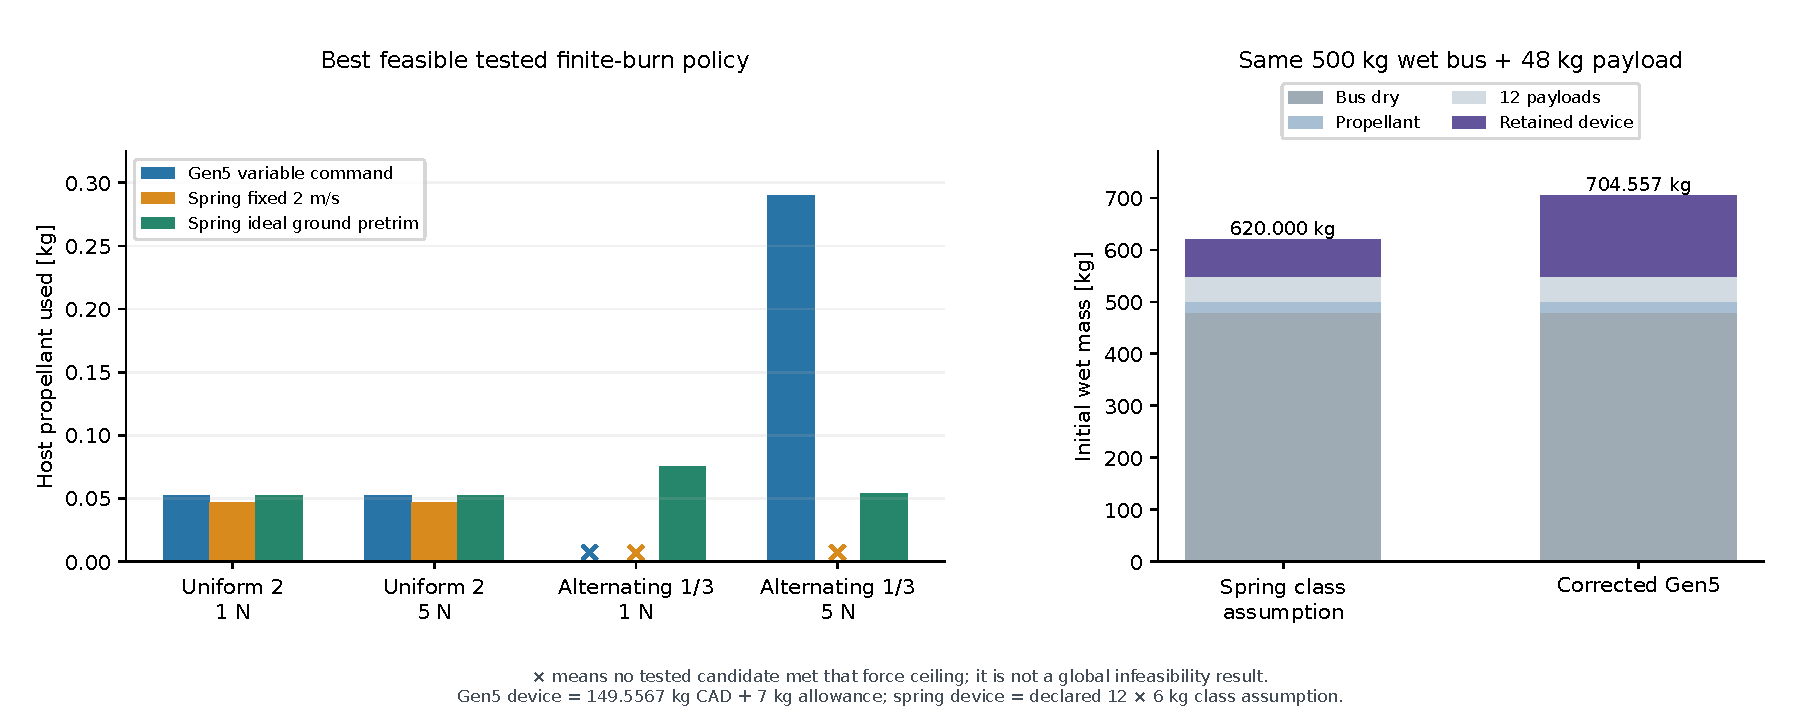
\includegraphics[width=0.92\textwidth]{MISSION_RESOURCES.pdf}
\caption{Current common-epoch mission resources. Ideal pretrim spring deployment provides a fair benchmark; a fixed-2 candidate above a force ceiling is a bounded policy result.}
\label{fig:mission}
\end{figure*}

\section{Discussion}
\subsection{A complete retained-carrier cycle}
The design result is a coupled cycle: storage, indexed transfer, positive docking, finite keeper opening, acceleration, unilateral separation, active arrest and powered return. Retaining the pallet makes the custody transition explicit and includes its mass in carrier dynamics. The same motor's ability to accelerate the payload and carrier does not automatically establish its ability to arrest the carrier in a shorter distance. The 210~mm allocation therefore forms a decisive constraint.

At 3~m/s the isolated kinetic-energy scale of the 13.128~kg retained carrier is approximately 59.1~J. The coupled simulation uses reduced masses, friction, source limits and finite force, yet this simple scale explains why post-release handling remains material at low speed. Ignoring the carrier after payload exit would omit both retained energy and a source-dependent operating requirement.

The source must support a feasible current transition as well as a peak current. Larger inductance reduces PWM ripple while delaying current decay. Regeneration then interacts with capacitor ESR and terminal-voltage headroom. The nominal/adverse inductance matrix addresses this interaction directly. The result supports the stated range for the chosen reference source; it does not establish a universal motor speed limit independent of source, control or mass.

\subsection{System trade and mission use}
The fixed banks allow twelve payloads to share one launch path, while the indexed mechanism creates common-path sequencing and fault-containment obligations. Retained magnets avoid payload-side motor hardware but increase carrier inertia. The complete assembly and source allowance impose a substantial dry burden. These tradeoffs must be compared against mission resources under equal boundaries.

A commanded release can reduce the host manoeuvre needed to create a payload state. That reduction must be assessed alongside dry mass, peak thrust, electrical recharge, handling time and attitude restoration. A propellant-use reduction alone does not establish lower wet mass, lower cost or a better customer service. The current reference is most relevant to a host already capable of sustained manoeuvring and repeated releases; a clearance-only deployment from an appropriate orbit has less need for variable velocity.

\subsection{Numerical credibility}
The verification methods constrain different numerical risks. Exact-solid checks address nominal part compatibility. Source-face integration checks finite magnetic-source implementation. Actual conductor FEM tests one current-distribution approximation. The audited time-step rerun checks the averaged current/source equations, limiting logic and event handling. Actual-chassis elasticity addresses the geometry and load path of the retained structure.

These agreements retain common physical assumptions. Uniform magnet polarization, idealized permeability, material properties, friction and circuit parasitics require correlation. Numerical residuals far below engineering tolerances indicate consistent calculations, not equivalent physical precision. The actual-chassis solve uses one accepted actual-geometry mesh for the bounded geometry-delta/gap decision and does not claim a continuum error bound.

\section{Scope and Prototype Development}
All VOLLEY results in this paper are computational. Native CAD and rendered geometry do not represent fabricated hardware. The source model is averaged with explicit ripple bounds and catalog-based allocations; it excludes transistor-resolved switching and measured layout parasitics. The current-distribution comparison covers one interior position under a permanent-field model. The chassis solve excludes magnets, adhesive, rollers, joints, stator supports and full host boundary conditions.

Clearance allocations are design bounds, and the end-frame stack represents rigid datums rather than elastic retainer contact. Contact-energy bounds use a declared rail/pad surrogate; they are not measured tip-off or a universal spacecraft property. The sharp-corner current-density maximum is a mesh observation without a converged physical hotspot interpretation. Local thermal recovery assumes repeated-cell diffusion between 450~s shots; feed capture excludes jam energy, guide play and measured restitution.

The mission families are synthetic requirements, with fixed-axis J2 and no drag or third bodies. Host propulsion and spring mass are class assumptions. Sampled two-window policies are not global optima or a conjunction-safety assessment. Native replay differences are numerical consistency measures rather than flight delivery accuracy.

The next validation step is an instrumented mixed 1U/3U Gen6 prototype. Static motor measurements should map force versus phase current and position. Conductor/source measurements should identify resistance, inductance and ESR. Transfer tests should measure pusher force, pallet pose and lock engagement rather than only endpoint arrival. Release/arrest tests should resolve payload/carrier speed, phase current, terminal voltage, separation timing and stop position. Repeated operation should correlate component temperatures and recharge state.

Environmental and payload compatibility require the selected host and spacecraft interfaces. Vibration, thermal-vacuum, magnetic exposure, electromagnetic compatibility, contamination and radiation are product-level questions beyond nominal geometric and source checks. Relevant environmental standards provide a framework for later verification \cite{gevs}. They are not evidence that the present reference is qualified.

Higher-speed development must carry forward the complete cycle. Payload energy grows as speed squared, while acceleration, stroke, source voltage, switching, arrest and failed-release consequences change together. A 1~km/s objective is future research in a different regime; it is not achieved by this study. The current low-speed reference supplies a reproducible basis for evaluating such changes.

\section{Conclusion}
The \acr\ reference defines a complete commanded electromagnetic deployment mechanism for twelve 4~kg 3U surrogates. Fixed banks, positive pushers and an indexed captive pallet supply an explicit custody path to the retained moving-magnet carrier. Eight released native/STEP states and 154 accepted motion/refinement checks support nominal geometric compatibility.

Finite force integration gives approximately 1.328~N/A active force and 1.399~N/A with represented returns. Independent source-face integration corroborates the active implementation and actual-current FEM differs by 0.172\% locally. All six principal 3~m/s cases pass audited 5~$\mu$s source/release/arrest review, supporting the upper end of the current computational 1--3~m/s range. Actual-chassis opposed-load closure is 0.286~mm, or 0.372~mm under the declared 1.3 multiplier.

The current common-state campaign closes the configured release families while showing no mass or fuel advantage over ideal pretrim spring deployment. The demonstrated distinction is commandability of the selected 1--3~m/s release range. The represented dry mass is 149.557~kg plus a separate 7~kg power/control allowance. The study establishes computational feasibility within its cases and explicit requirements for physical validation, without an installed-mass or qualification claim. Gen6 development should correlate the dominant mechanical, electrical and thermal interfaces in an instrumented mixed-size prototype.

\section*{Acknowledgment}
The authors acknowledge the Department of Mechanical Engineering at Symbiosis Institute of Technology and project guide Vikas Gulia. FreeCAD, Open CASCADE, Blender, NumPy, magpylib, Gmsh and CalculiX support the stated computational methods. Their use does not imply endorsement of the design.

\section*{Reproducibility}
The accompanying academic source package includes local figures, an asset map and controlled evidence records. The full engineering package retains native/STEP states, model inputs, solver outputs and source hashes under configuration VOLLEY-G5-ACR1. Mechanical builder identity begins \texttt{e1179e886282}, actual-chassis BREP \texttt{d4b53d520c1bc}, and principal shot source \texttt{560088cb2a05}; complete digests are in the evidence maps. The source package is an unsubmitted manuscript; no publication acceptance is represented.

\begin{thebibliography}{99}
\bibitem{jssod} JAXA, \emph{JEM Payload Accommodation Handbook}, vol. 8, Small Satellite Deployment Interface Control Document, via UNOOSA KiboCUBE.
\bibitem{cds} California Polytechnic State University, \emph{CubeSat Design Specification}, rev. 14.1, 2022.
\bibitem{foster} C. Foster \emph{et al.}, ``Constellation phasing with differential drag on Planet Labs satellites,'' \emph{J. Spacecraft Rockets}, vol. 55, no. 2, 2018.
\bibitem{vallado} D. A. Vallado, \emph{Fundamentals of Astrodynamics and Applications}, 4th ed. Microcosm Press, 2013.
\bibitem{stacked} Y. Zhao, H. Yue, X. Mu, X. Yang, and F. Yang, ``Design and analysis of a new deployer for the in-orbit release of multiple stacked CubeSats,'' \emph{Remote Sensing}, vol. 14, no. 17, art. 4205, 2022, doi:10.3390/rs14174205.
\bibitem{storage} Y. Zhao \emph{et al.}, ``Simulation analysis and experimental verification of the transport characteristics of a high-volume CubeSat storage device,'' \emph{Aerospace}, vol. 12, no. 6, art. 466, 2025, doi:10.3390/aerospace12060466.
\bibitem{feng} H. Feng, Y. Yang, and Y. Wu, ``Design and reachable domain analysis of on-orbit electromagnetic launcher for CubeSats,'' \emph{Int. J. Aerospace Eng.}, art. 3000765, 2025, doi:10.1155/ijae/3000765.
\bibitem{halbach} K. Halbach, ``Design of permanent multipole magnets with oriented rare earth cobalt material,'' \emph{Nucl. Instrum. Methods}, vol. 169, pp. 1--10, 1980.
\bibitem{end} H. Yamaguchi and M. Morishita, ``End effects of Halbach field magnet-type linear motor,'' \emph{Electrical Engineering in Japan}, vol. 216, no. 4, art. e23450, 2023, doi:10.1002/eej.23450. Selected Japanese-original passages examined: \emph{IEEJ Trans. Industry Applications}, vol. 143, no. 8, pp. 570--578, 2023, doi:10.1541/ieejias.143.570.
\bibitem{magpylib} M. Ortner and L. G. Coliado Bandeira, ``Magpylib: A free Python package for magnetic field computation,'' \emph{SoftwareX}, vol. 11, art. 100466, 2020, doi:10.1016/j.softx.2020.100466.
\bibitem{eaton} Eaton, \emph{TV Supercapacitors: Cylindrical Cells}, manufacturer data sheet, captured source SHA256 beginning \texttt{eaddcdbd008e}.
\bibitem{mosfet} Infineon Technologies, \emph{IRFP4668PbF Power MOSFET}, manufacturer data sheet, captured source SHA256 beginning \texttt{117c4a335eea}.
\bibitem{driver} Texas Instruments, \emph{UCC21520 Isolated Dual-Channel Gate Driver}, manufacturer data sheet, captured source SHA256 beginning \texttt{9fa909613e47}.
\bibitem{gmsh} C. Geuzaine and J.-F. Remacle, ``Gmsh: A 3-D finite element mesh generator with built-in pre- and post-processing facilities,'' \emph{Int. J. Numer. Methods Eng.}, vol. 79, no. 11, pp. 1309--1331, 2009, doi:10.1002/nme.2579.
\bibitem{ccx} G. Dhondt and K. Wittig, \emph{CalculiX}, finite-element software and user documentation, ver. 2.23.
\bibitem{orekit} Orekit Project and Hipparchus Project, \emph{Orekit 13.1.6} and \emph{Hipparchus 4.0.3}, orbital dynamics and numerical libraries; captured runtime and JAR identities accompany G5-MISSION-01.
\bibitem{gevs} NASA, \emph{General Environmental Verification Standard}, GSFC-STD-7000A, 2013.
\end{thebibliography}
\end{document}
